In this chapter sample theory and its importance when converting an analog audio signal to a digital audio signal along with its complications is treated.
%\section{The frequency domain}
%The following sections look at functions in both the \textit{time}- and \textit{frequency} domains and utilizes the advantages of these different visualizations. To express a function of time as a function of frequency the \textit{Fourier transform} is used. The transform decomposes a periodic function $A$ of time $t$ into an amplitude valued function $\hat{A}$ of frequency $\omega$ and shows which amplitudes of frequencies of different sinusoids are present in the signal. The mathematical background for the Fourier transform is reserved for chapter \ref{ch5} - this chapter will make do with the graphical explanation in figures \ref{fig:time} and \ref{fig:freq}. Notice the both real and imaginary amplitudes of $\hat{A}$.
%\begin{figure}[H]
%\centering
%\begin{minipage}{0.49\textwidth}
%\centering
%\begin{tikzpicture}[scale=0.8]
%\begin{axis}[
%axis lines=middle,
%xtick={-3.14159,3.14159},
%xticklabels={$-\pi$,$\pi$},
%ytick={-1.5,1.5}
%,xmin=-4.25
%,xmax=4.25
%,ymin=-1.75
%,ymax=1.75,
%samples=50]
%\addplot[red][domain=-3.14159:3.14159] {sin(deg(x))+(1/2)*cos(deg(2*x))};
%\end{axis}
%\end{tikzpicture}
%\caption{Graph of $f(x)=\sin x + \frac{1}{2} \cos 2x$ in the time domain.}
%\label{fig:time}
%\end{minipage}
%\centering
%\begin{minipage}{0.49\textwidth}
%\centering
%\begin{tikzpicture}[scale=0.8]
%\begin{axis}[
%axis lines=middle,
%xtick={-6.28318,-3.14159,3.14159,6.28318},
%xticklabels={$-2\pi$,$-\pi$,$\pi$,$2\pi$},
%ytick={-1.5,1.5},
%xmin=-6.75,
%xmax=6.75,
%ymin=-1.75,
%ymax=1.75]
%\draw[->][red](axis cs:6.28318,0)--(axis cs:6.28318,0.62665);
%\draw[->][red](axis cs:-6.28318,0)--(axis cs:-6.28318,0.62665);
%\draw[->][blue](axis cs:3.14159,0)--(axis cs:3.14159,1.2533);
%\draw[->][blue](axis cs:-3.14159,0)--(axis cs:-3.14159,1.2533);
%\end{axis}
%\end{tikzpicture}
%\caption{Graph of $\hat{f}$ in the frequency domain. Red = real, blue = imaginary.}
%\label{fig:freq}
%\end{minipage}
%\end{figure}
%The above figures illustrate the continuous Fourier transform. The transform can be discretized to the discrete Fourier transform, which is crucial, when working with sampled signals. This is likewise covered in chapter \ref{ch5}.
\section{Sampling} \label{sec:sampling}
In this section sampling will be defined mathematically, which allows for a frequency analysis leading to the establishment of the important \textit{Sampling Theorem}.
\\ \\
Sampling is the process of representing a time-continuous signal by a sequence of values. Doing so converts the time-continuous signal into a time-discrete signal $x(n)$ \cite{pelgrom}. Sampling is usually done with digitalization of the signal in mind, and this requires the signal to be discretized in amplitude, too.$^[$\footnote{$x(n)$ is merely discrete in time and will be sufficient for the following mathematical representation of sampling.}$^]$ When discretized in both time and amplitude the signal is referred to as $x[n]$. The relation between a continuous function $x_c(t)$ and the discrete funtion $x(n)$ obtained by sampling $x_c(t)$ is described by
\begin{align} \label{eq:sampling_principle}
x(n)=x_c(nT_s),
\end{align}

where $n \in \mathbb{Z}$ and the \textit{sampling period} $T_s$ (the time between two consecutive samples) is determined by the \textit{sampling frequency} $f_s$ (samples pr. second). The relation between $T_s$, $f_s$ and the times of samples is described by \cite{pelgrom}:
\begin{align} \label{eq:sample_freq}
\dfrac{n}{f_s} = nT_s,
\end{align}

where $n$ is the number of samples and $nT_s$ are the points in time of sampling.
\\ \\
To describe sampling mathematically the \textit{Dirac delta} function is introduced.

\begin{definition}[Dirac delta function]$^[$\footnote{The Dirac delta function is defined as a distribution as no function satisfies the properties in definition \ref{def:dirac}. This definition is therefore non-rigorous but sufficient for the purposes of this section.}$^]$ \label{def:dirac}
The Dirac delta function is the function $\delta$ satisfying
\begin{align}
\int_{-\infty}^{\infty} \! f(t)\delta(t-t_0) \, dt=f(t_0).\phantom{mm}
\end{align}
\end{definition}

The Dirac delta function is sometimes interpreted as a function $\delta(t)$ satisfying $\delta(t)=0$ for $t\neq 0$ and $\int_{-\infty}^{\infty}\!\delta(t)\,dt=1$.
\\ \\
In signal processing the similar \textit{Kronecker delta sequence} is often used as a unit impulse.
\begin{definition}[Kronecker delta sequence]\label{def:kronecker}
The Kronecker delta sequence is $\{\delta_n\}_{n\in\mathbb{N}}$, where
\begin{align}
\delta_n=
\begin{cases}1,\text{ for }n=0\\
0,\text{ otherwise}
\end{cases}\phantom{mm}n\in\mathbb{Z}
\end{align}
\end{definition}

Depending on the context either the Dirac or the Kronecker delta may be used. In the context of this section, the Dirac delta is preferred, as it makes the mathematical analysis of sampling easier.\\\\
Summing an infinite number of Dirac functions shifted at equally spaced time intervals $nT_s$ as in \eqref{eq:dirac_sum} produces a constant function of equidistant Dirac pulses called a Dirac comb, which is an infinite sequence of Dirac pulses \cite{DTSP}:
\begin{align} \label{eq:dirac_sum}
s(t)=\sum_{n=-\infty}^{\infty}\delta(t-nT_s)
\end{align}

A Dirac comb is seen in figure \ref{fig:dirac_comb}.
\begin{figure}[H]
\centering
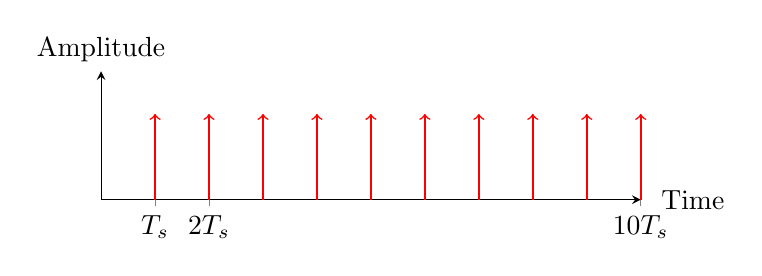
\begin{tikzpicture}
\begin{axis}[
unit vector ratio*=1 1 1,
axis lines=middle,
clip=false,
xmax=10,
xmin=0,
ymax=2.38,
ymin=0,
ytick=\empty,
xtick={1,2,10},
xticklabels={$T_s$,$2T_s$,$10T_s$},
x label style={at={(axis cs:10.2,0)},anchor=west},
y label style={at={(axis cs:0,2.38)},anchor=south},
xlabel=Time,
ylabel=Amplitude]
\draw[->,line width=0.2mm,red](axis cs:1,0)--(axis cs:1,1.59);
\draw[->,line width=0.2mm,red](axis cs:2,0)--(axis cs:2,1.59);
\draw[->,line width=0.2mm,red](axis cs:3,0)--(axis cs:3,1.59);
\draw[->,line width=0.2mm,red](axis cs:4,0)--(axis cs:4,1.59);
\draw[->,line width=0.2mm,red](axis cs:5,0)--(axis cs:5,1.59);
\draw[->,line width=0.2mm,red](axis cs:6,0)--(axis cs:6,1.59);
\draw[->,line width=0.2mm,red](axis cs:7,0)--(axis cs:7,1.59);
\draw[->,line width=0.2mm,red](axis cs:8,0)--(axis cs:8,1.59);
\draw[->,line width=0.2mm,red](axis cs:9,0)--(axis cs:9,1.59);
\draw[->,line width=0.2mm,red](axis cs:10,0)--(axis cs:10,1.59);
\end{axis}
\end{tikzpicture}
\caption{Dirac comb $s(t)$.}
\label{fig:dirac_comb}
\end{figure}
Multiplying a continuous signal with \eqref{eq:dirac_sum} and using the properties of the Dirac function, then \eqref{eq:sampling} is obtained:
\begin{align} \label{eq:sampling}
x_s(t)&=x_c(t)s(t)\nonumber \\
&=x_c(t)\sum_{n=-\infty}^{\infty}\delta(t - nT_s)\nonumber \\
&=\sum_{n=-\infty}^{\infty}x_c(t)\delta(t - nT_s)\nonumber\\
&=\sum_{n=-\infty}^{\infty}x_c(nT_s)\delta(t - nT_s).
\end{align}

\eqref{eq:sampling} is a mathematical representation of sampling of the continuous function $x_c(t)$ into the function $x_s(t)$ \cite{DTSP}. This process is seen in figure \ref{fig:signal1}, where a signal is shown, and figure \ref{fig:sampling_comb}, where the signal is sampled by multiplication with a Dirac comb.

\begin{figure}[H]
\centering
\begin{tikzpicture}
\begin{axis}[
clip=false,
unit vector ratio*=1 1 1,
axis lines=middle,
xmax=10,
xtick={5,10},
xticklabels={$\pi$,$2\pi$},
xmin=0,
ymax=2.38,
ymin=-2.38,
ytick=\empty,
x label style={at={(axis cs:11,0)},anchor=north},
y label style={at={(axis cs:0,2.5)},anchor=south},
xlabel=Time,
ylabel=Amplitude]
\addplot[red,domain=0:10,samples=50,line width=0.2mm]{10/6.2831*sin((2*3.1415)/10*deg(x))};
\end{axis}
\end{tikzpicture}
\caption{Signal $x_c(t)=\sin(x)$.}
\label{fig:signal1}
\end{figure}
\begin{figure}[H]
\centering
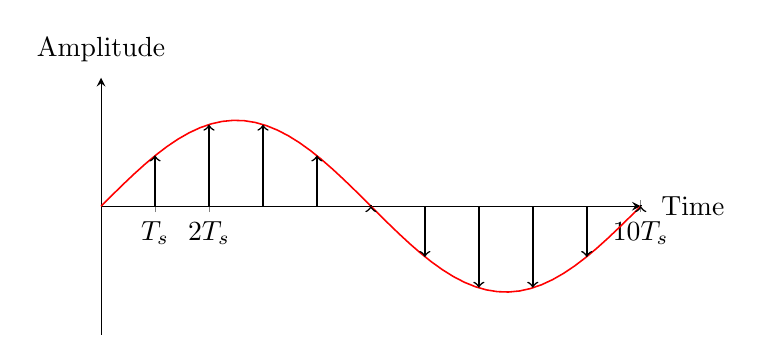
\begin{tikzpicture}
\begin{axis}[
clip=false,
unit vector ratio*=1 1 1,
axis lines=middle,
xmin=0,
xmax=10,
ymin=-2.38,
ymax=2.38,
ytick=\empty,
xtick={1,2,10},
xticklabels={$T_s$,$2T_s$,$10T_s$},
x label style={at={(axis cs:10.2,0)},anchor=west},
y label style={at={(axis cs:0,2.5)},anchor=south},
xlabel=Time,
ylabel=Amplitude]
\addplot[red,samples=50,domain=0:10,line width=0.2mm]{10/6.2831*sin(6.2831/10*deg(x))};
\draw[->,line width=0.2mm](axis cs:1,0)--(axis cs:1,0.94);
\draw[->,line width=0.2mm](axis cs:2,0)--(axis cs:2,1.51);
\draw[->,line width=0.2mm](axis cs:3,0)--(axis cs:3,1.51);
\draw[->,line width=0.2mm](axis cs:4,0)--(axis cs:4,0.94);
\draw[->,line width=0.2mm](axis cs:5,0)--(axis cs:5,0);
\draw[->,line width=0.2mm](axis cs:6,0)--(axis cs:6,-0.94);
\draw[->,line width=0.2mm](axis cs:7,0)--(axis cs:7,-1.51);
\draw[->,line width=0.2mm](axis cs:8,0)--(axis cs:8,-1.51);
\draw[->,line width=0.2mm](axis cs:9,0)--(axis cs:9,-0.94);
\draw[->,line width=0.2mm](axis cs:10,0)--(axis cs:10,0);
\end{axis}
\end{tikzpicture}
\caption{Signal $x_c(t)=\sin(x)$ sampled at $f_s=10$ Hz by multiplication with a Dirac comb $s(t)=\sum_{-\infty}^{\infty}\delta(t-\frac{n}{10\pi})$.}
\label{fig:sampling_comb}
\end{figure}

Although \eqref{eq:sampling} mathematically describes sampling (as in converting a time-continuous signal to a time-discrete), then $x_s(t) \neq x[n]$ as $x_s(t)$ is not discretized in amplitude whereas $x[n]$ is. Although $x_s(t) \neq x[n]$ \eqref{eq:sampling} will be useful in the upcoming appliance of the Fourier transform.
%\paragraph{Example of sampling} Sampling a ball following the arc shown in figure \ref{fig:ball_cont} results in the plotted points in figure \ref{fig:ball_disc}. As such the balls path is illustrated with discrete points along the path.
%\begin{figure}[H]
%\centering
%\begin{minipage}{0.49\textwidth}
%\centering
%\begin{tikzpicture}[scale=1.4]
%\draw[->] (-0.25,0) -- (4.25,0) node[right] {$x$};
%\draw[->] (0,-0.25) -- (0,2) node[above] {$y$};
%\draw[scale=1,domain=0:4,smooth,variable=\x,red] plot ({\x},{-0.25*\x*\x+\x});
%\end{tikzpicture}
%\caption{Trajectory of a ball described by the time continuous function $x_c(t)$. In continuous time the trajectory is smooth.}
%\label{fig:ball_cont}
%\end{minipage}
%\centering
%\begin{minipage}{0.49\textwidth}
%\centering
%\begin{tikzpicture}[scale=1.4]
%\draw[->] (-0.25,0) -- (4.25,0) node[right] {$x$};
%\draw[->] (0,-0.25) -- (0,2) node[above] {$y$};
%\draw(0,0) node {\textbullet};
%\draw(0.5,0.4375) node {\textbullet};
%\draw(1,0.75) node {\textbullet};
%\draw(1.5,0.9375) node {\textbullet};
%\draw(2,1) node {\textbullet};
%\draw(2.5,0.9375) node {\textbullet};
%\draw(3,0.75) node {\textbullet};
%\draw(3.5,0.4375) node {\textbullet};
%\draw(4,0) node {\textbullet};
%\end{tikzpicture}
%\caption{Trajectory of a ball described by the time discrete function $x[n]$. The trajectory consists of samples of $x_c(t)$.}
%\label{fig:ball_disc}
%\end{minipage}
%\end{figure}
\subsection{Frequency representation of sampling}
Studying $x_s(t)$ and $s(t)$ in the frequency domain leads to some important conclusions about sampling. Before $s(t)$ is Fourier transformed it is expanded into its Fourier series:
%Firstly the Dirac delta function is Fourier transformed - the result follows directly from the definition of the Fourier transform and definition \ref{def:dirac}:
%\begin{align}\label{eq:fourier_delta}
%\mathcal{F}[\delta(t)]=\Delta(\omega)=\int_{-\infty}^{\infty}\!\delta(t)\mathrm{e}^{-j\omega t}\,dt=\mathrm{e}^0=1
%\end{align}
%\eqref{eq:fourier_delta} shows, that the Fourier transform of $\delta$ is a constant function of value 1. The Fourier transform of the Dirac comb $s(t)$ is given by expanding $s(t)$ with its Fourier series.
\begin{align*}
s(t)&=\sum_{n=-\infty}^{\infty}\delta(t-nT_s) \\
&=\sum_{n=-\infty}^{\infty}c_n\mathrm{e}^{j nt/T_s}.
\end{align*}

Calculation of the $c_n$ coefficients gives
\begin{align*}
c_n &= \dfrac{1}{T_s} \int_{t_0}^{t_0+T_s} \! s(t) \mathrm{e}^{-jnt/T_s} \, dt = \dfrac{1}{T_s} \int_{-T_s/2}^{T_s/2} \! \delta(t) \mathrm{e}^{-jnt/T_s} \, dt \\
&= \dfrac{1}{T_s}\mathrm{e}^0 = \dfrac{1}{T_s}.
\end{align*}

And so the Fourier series of $s(t)$ is
\begin{align}\label{eq:dirac_series}
s(t) = \dfrac{1}{T_s} \sum_{n=-\infty}^{\infty} \mathrm{e}^{jnt/T_s} \phantom{mm} \forall n \ \in \mathbb{Z}.
\end{align}

\eqref{eq:dirac_series} shows that the Fourier series of $s(t)$ is merely an inifite number of phase shifted sines of equal frequencies summed. This makes the following Fourier transform easy:
\begin{align} \label{eq:fourier_comb1}
\mathcal{F}\{s(t)\}(\omega) &= \dfrac{1}{T_s} \mathcal{F}\left\{\sum_{n=-\infty}^{\infty} \mathrm{e}^{jnt/T_s} \right\} (\omega) \nonumber \\
&= \frac{1}{T_s} \int_{-\infty}^{\infty} \! \sum_{n=-\infty}^{\infty} \mathrm{e}^{jnt/T_s} \mathrm{e}^{-j\omega t} \, dt \nonumber \\
&= \frac{1}{T_s} \sum_{n=-\infty}^{\infty} \int_{-\infty}^{\infty} \! \mathrm{e}^{-j(\omega-n/T_s)t} \, dt
\end{align}

\eqref{eq:fourier_comb1} is the Fourier transform of a constant function $f(t) = 1$. As $f(t) = 1 \notin \mathcal{L}^1$ its Fourier transform is not well-defined. It can however be shown that $\mathcal{F}\{1\}(\omega) = \delta(\omega)$ $^[$\footnote{This relates to the Dirac delta function being a distribution and will not be discussed here.}$^]$, and so \eqref{eq:fourier_comb1} evaluates to
\begin{align} \label{eq:fourier_comb2}
\frac{1}{T_s} \sum_{n=-\infty}^{\infty} \int_{-\infty}^{\infty} \! \mathrm{e}^{-j(\omega-n/T_s)t} \, dt &= \dfrac{1}{T_s}\sum_{n=-\infty}^{\infty} \delta(\omega-\frac{n}{T_s}) \nonumber \\
&= \dfrac{1}{T_s} \sum_{n=-\infty}^{\infty} \delta(\omega-n\omega_s).
\end{align}

\eqref{eq:fourier_comb2} shows that the Fourier transform of $s(t)$ results in another Dirac comb in the frequency domain with pulses seperated by $\omega_s$.
Calculating the Fourier transform of \eqref{eq:sampling} uses \eqref{eq:fourier_comb2} and the fact that \eqref{eq:sampling} is a product of two functions, which is a convolution in the frequency domain:
\begin{align} \label{eq:samp_freq}
\mathcal{F}\{x_s(t)\}(\omega) &= \mathcal{F}\{x_c(t)s(t)\} \nonumber \\
&= \dfrac{1}{T} \sum_{k=-\infty}^{\infty} X_c(t)(\omega) * S(\omega) \nonumber \\
X_s(\omega)&=\frac{1}{T}\sum_{k=-\infty}^{\infty}X_c(\omega-k\omega_s)
\end{align}

Just as \eqref{eq:sampling} mathematically samples $x_c(t)$ in the time domain, \eqref{eq:samp_freq} mathematically samples $X_c(\omega)$ in the frequency domain at a rate of $\omega_s$. The following section draws conlusions regarding sampling frequencies by studying $X_c(\omega)$.

\subsection{Aliasing} \label{sec:aliasing}
\textit{Aliasing} is a consequence of not sampling at a sufficiently high sampling frequency $f_s$ which results in the continuous signal $x_c(t)$ being non-reconstructable from the sampled signal $x_s(t)$. In this discussion \textit{bandlimited} signals are of interest.

\paragraph{Bandlimited signal}
A signal is bandlimited if the signal contains no frequencies higher than some frequency $\omega_N$, which means that $F(\omega) = 0$ for $|\omega|>\omega_N$ \cite{FAA}.
\\\\
From \eqref{eq:samp_freq} it is seen that $X_s(\omega)$ consists of copies of $X_c$ repeated at whole multiples of $\omega_s$ on both sides of the origin, which is shown in figure \ref{fig:copies}.
\begin{figure}[H]
\centering
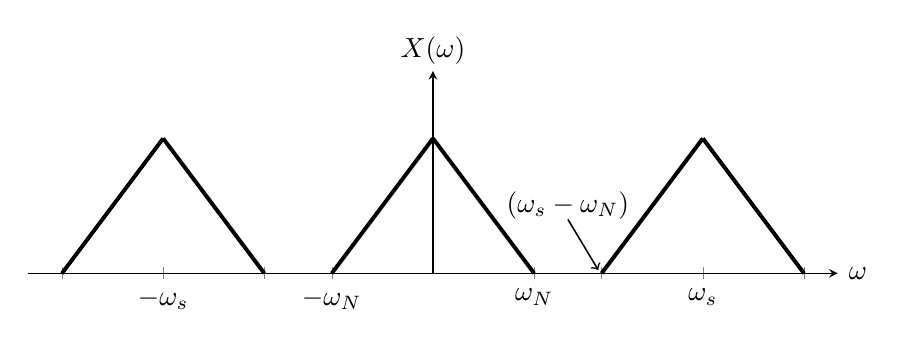
\begin{tikzpicture}
\begin{axis}[
scale=1.5,
clip=false,
unit vector ratio*=1 1 1,
axis lines = middle,
xtick={-4,4,1.5,-1.5,2.5,5.5,-5.5,-2.5},
xticklabels={$-\omega_s$,$\omega_s$,$\omega_N$,$-\omega_N$},
ytick=\empty,
xmin=-6,
xmax=6,
ymin=0,
ymax=3]
\node at (axis cs:2,1) {$(\omega_s-\omega_N$)};
\draw[->,line width=0.2mm] (axis cs:2,0.8)--(axis cs:2.45,0.05);
\draw[line width=0.5mm](axis cs:0,2)--(axis cs:1.5,0);
\draw[line width=0.5mm](axis cs:0,2)--(axis cs:-1.5,0);
\draw[line width=0.5mm](axis cs:4,2)--(axis cs:5.5,0);
\draw[line width=0.5mm](axis cs:4,2)--(axis cs:2.5,0);
\draw[line width=0.5mm](axis cs:-4,2)--(axis cs:-5.5,0);
\draw[line width=0.5mm](axis cs:-4,2)--(axis cs:-2.5,0);
\node at(axis cs:0,3.3){$X(\omega)$};
\node at(axis cs:6.3,0){$\omega$};
	\end{axis}
\end{tikzpicture}
\caption{Signal bandlimited by $\omega_N$ sampled at $\omega_s$ in the frequency domain. Copies of $X_c$ are seen at whole multiples of $\omega_s$.}
\label{fig:copies}
\end{figure}

It is clear from figure \ref{fig:copies} that if $\omega_s-\omega_N\geq \omega_N\Rightarrow \omega_s\geq 2\omega_N$ there is no overlap of the copies of $X_c$. With an ideal low pass filter  a single isolated copy (centered around the origin) can be picked out, and the inverse Fourier transform used to recreate the time domain representation of the signal. If, however, $\omega_s-\omega_N\leq \omega_N\Rightarrow \omega_s\leq 2\omega_N$ the copies will overlap as seen in figure \ref{fig:overlap}. This is called aliasing. When a signal is aliased it is not possible to pick out a single copy of the sampled signal in the frequency domain, which results in $x_c(t)$ not being reconstructable from $x_s(t)$. This makes aliasing unwanted in the context of representing a continuous signal as a discrete set of values \martin{Er ikke så glad for denne sætning. Det lyder lidt som om, at man godt kan ønske spejling. \textregistered}.

\begin{figure}[H]
\centering
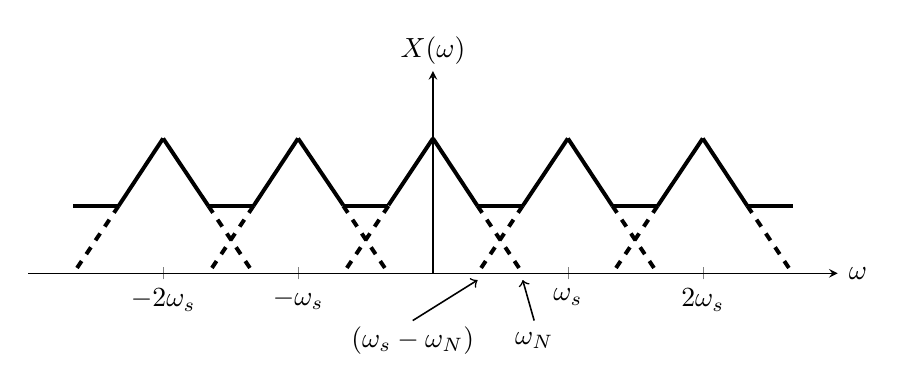
\begin{tikzpicture}
\begin{axis}[
clip=false,
scale=1.5,
unit vector ratio*=1 1 1,
axis lines = middle,
xtick={-2,2,-4,4},
xticklabels={$-\omega_s$,$\omega_s$,$-2\omega_s$,$2\omega_s$},
ytick=\empty,
xmin=-6,
xmax=6,
ymin=0,
ymax=3]
\draw[line width=0.5mm](axis cs:0,2)--(axis cs:0.66,1);
\draw[line width=0.5mm](axis cs:2,2)--(axis cs:1.33,1);
\draw[line width=0.5mm](axis cs:0.66,1)--(axis cs:1.33,1);
\draw[line width=0.5mm](axis cs:2,2)--(axis cs:2.66,1);
\draw[line width=0.5mm](axis cs:2.66,1)--(axis cs:3.33,1);
\draw[line width=0.5mm](axis cs:3.33,1)--(axis cs:4,2);
\draw[line width=0.5mm](axis cs:4,2)--(axis cs:4.66,1);
\draw[line width=0.5mm](axis cs:0,2)--(axis cs:-0.66,1.01);
\draw[line width=0.5mm](axis cs:-2,2)--(axis cs:-1.33,1.01);
\draw[line width=0.5mm](axis cs:-0.66,1)--(axis cs:-1.33,1);
\draw[line width=0.5mm](axis cs:-2,2)--(axis cs:-2.66,1);
\draw[line width=0.5mm](axis cs:-2.66,1)--(axis cs:-3.33,1);
\draw[line width=0.5mm](axis cs:-3.33,1)--(axis cs:-4,2);
\draw[line width=0.5mm](axis cs:-4,2)--(axis cs:-4.66,1);
\draw[line width=0.5mm](axis cs:-4.66,1.)--(axis cs:-5.33,1);
\draw[line width=0.5mm](axis cs:4.66,1)--(axis cs:5.33,1);
\draw[line width=0.5mm,dashed](axis cs:0.66,1)--(axis cs:1.33,0);
\draw[line width=0.5mm,dashed](axis cs:1.33,1)--(axis cs:0.66,0);
\draw[line width=0.5mm,dashed](axis cs:-0.66,1)--(axis cs:-1.33,0);
\draw[line width=0.5mm,dashed](axis cs:-1.33,1)--(axis cs:-0.66,0);
\node at(axis cs:-0.3,-1){($\omega_s-\omega_N$)};
\draw[->,line width=0.2mm](axis cs:-0.3,-0.7)--(axis cs:0.66,-0.1);
\node at(axis cs:1.5,-1){$\omega_N$};
\draw[->,line width=0.2mm](axis cs:1.5,-0.7)--(axis cs:1.33,-0.1);
\draw[line width=0.5mm,dashed](axis cs:2.66,1)--(axis cs:3.33,0);
\draw[line width=0.5mm,dashed](axis cs:3.33,1)--(axis cs:2.66,0);
\draw[line width=0.5mm,dashed](axis cs:4.66,1)--(axis cs:5.33,0);
\draw[line width=0.5mm,dashed](axis cs:-2.66,1)--(axis cs:-3.33,0);
\draw[line width=0.5mm,dashed](axis cs:-3.33,1)--(axis cs:-2.66,0);
\draw[line width=0.5mm,dashed](axis cs:-4.66,1)--(axis cs:-5.33,0);
\node at(axis cs:0,3.3){$X(\omega)$};
\node at(axis cs:6.3,0){$\omega$};
\end{axis}
\end{tikzpicture}
\caption{Signal bandlimited by $\omega_N$ sampled at $\omega_s<2\omega_N$ in the frequency domain - the copies of $X_c$ overlap.}
\label{fig:overlap}
\end{figure}

An extreme case of aliasing happens if the frequencies of two different signals differ from some whole multiple of $f_s$ by the same amount. The sequence of samples for the two signals will then be identical. An example of this is shown in figures  \ref{fig:aliasing1} and \ref{fig:aliasing2}, where two sine waves of different frequencies are sampled with the same sampling frequency $f_s$.
\begin{figure}[H]
\centering
\begin{subfigure}{0.49\textwidth}
\centering
\begin{tikzpicture}[scale=0.8]
\begin{axis}[
axis lines=middle,
xtick={6.28138},
xticklabels={1 s},
ytick={-1,1}
,xmin=-.25
,xmax=6.5
,ymin=-1.25
,ymax=1.25
,samples=50]
\addplot[red][domain=0:6.28318]{sin(deg(x))};
\node at (axis cs:0,0) {\textbullet};
\node at (axis cs:0.6918,0.6428) {\textbullet};
\node at (axis cs:1.3963,0.9848) {\textbullet};
\node at (axis cs:2.0944,0.8660) {\textbullet};
\node at (axis cs:2.7925,0.3420) {\textbullet};
\node at (axis cs:3.4907,-0.3420) {\textbullet};
\node at (axis cs:4.1888,-0.8660) {\textbullet};
\node at (axis cs:4.8869,-0.9848) {\textbullet};
\node at (axis cs:5.5850,-0.6428) {\textbullet};
\node at (axis cs:6.2832,0) {\textbullet};
\end{axis}
\end{tikzpicture}
\caption{Sine wave of frequency $f=1$ Hz sampled at $f_s=9$ Hz.}
\label{fig:aliasing1}
\end{subfigure}
\begin{subfigure}{0.49\textwidth}
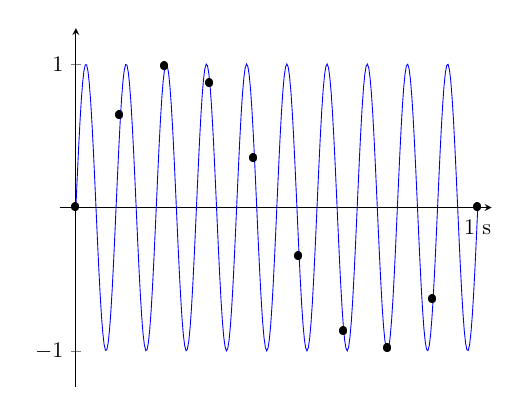
\begin{tikzpicture}[scale=0.8]
\begin{axis}[
axis lines=middle,
xtick={6.28138},
xticklabels={1 s},
ytick={-1,1}
,xmin=-.25
,xmax=6.5
,ymin=-1.25
,ymax=1.25
,samples=300]
\addplot[blue][domain=0:6.28138]{sin(deg(10*x))};
\node at (axis cs:0,0){\textbullet};
\node at (axis cs:0.6918,0.6428){\textbullet};
\node at (axis cs:1.3963,0.9848){\textbullet};
\node at (axis cs:2.0944,0.8660){\textbullet};
\node at (axis cs:2.7925,0.3420){\textbullet};
\node at (axis cs:3.4907,-0.3420){\textbullet};
\node at (axis cs:4.1888,-0.8660){\textbullet};
\node at (axis cs:4.8869,-0.9848){\textbullet};
\node at (axis cs:5.5850,-0.6428){\textbullet};
\node at (axis cs:6.2832,0){\textbullet};
\end{axis}
\end{tikzpicture}
\caption{Sine wave of frequency $f=10$ Hz sampled at $f_s=9$ Hz.}
\label{fig:aliasing2}
\end{subfigure}
\caption{2 sine waves of different frequencies sampled with the same sampling frequency.}
\label{fig:aliasingcol}
\end{figure} 

As figure \ref{fig:aliasingcol} shows, sampling the signal shown in figure \ref{fig:aliasing2} with $f_s = 9$ Hz could result in the signal being reconstructed as the signal shown in figure \ref{fig:aliasing1}. Therefore, the reconstructability of $x_c$ from $x_s$ depends on the relation between $f_s$ and $\omega_N$, which leads to the central \textit{Sampling Theorem} \cite{page 230, FAA}.

\begin{theorem}[The Sampling Theorem] \label{sampling_theorem}
Let $f \in L^2$ and $F(\omega) = 0$ for $|\omega| \geq \omega_N$ (that is, $f$ is bandlimited). Then $f$ is completely determined by its values at the points $t_n = \frac{n \pi}{\omega_N}$, $n=0,\pm 1,\pm 2,\ldots$:
\begin{align*}
f(t) = \sum_{n=-\infty}^{\infty} f \left( \dfrac{n\pi}{\omega_N} \right) \mathrm{sinc}(\omega_N t - n\pi),
\end{align*}

where
\begin{align}
\mathrm{sinc}(x) = \frac{\sin(x)}{x}.
\end{align}
\end{theorem}

\begin{proof}
The inverse Fourier transform of $f$ is written according to definition \ref{def:InverseFourier_trans}:
\begin{align} \label{eq:proof1}
f(t) = \dfrac{1}{2\pi} \int_{-\omega_N}^{\omega_N} \! F(\omega)\mathrm{e}^{j\omega t} \, d\omega.
\end{align}

$F$ is expanded into its Fourier series on $[-\omega_N,\omega_N]$, and the negative index $-n$ is used:
\begin{align*}
F(\omega) = \sum_{n=-\infty}^{\infty} c_{-n} \mathrm{e}^{-jn\pi\omega/\omega_N}, \phantom{mm} \omega \in [-\omega_N,\omega_N],
\end{align*}

where $c_{-n}$ is given by
\begin{align*}
c_{-n} &= \dfrac{1}{2\omega_N} \int_{-\omega_N}^{\omega_N} \!F(\omega) \mathrm{e}^{jn\pi\omega/\omega_N} \, d\omega \\
&= \dfrac{\pi}{\omega_N} f \left( \dfrac{n\pi}{\omega_N}\right).
\end{align*}

Then \eqref{eq:proof1} can be written as
\begin{align} \label{eq:limit}
f(t) &= \dfrac{1}{2\pi} \int_{-\omega_N}^{\omega_N} F(\omega) \mathrm{e}^{j\omega t} d\omega = \dfrac{1}{2\pi} \int_{-\omega_N}^{\omega_N} \sum_{n=-\infty}^{\infty} \dfrac{\pi}{\omega_N} f \left( \dfrac{n\pi}{\omega_N}\right) \mathrm{e}^{-jn\pi\omega/\omega_N} \mathrm{e}^{j\omega t} d\omega \nonumber \\
&= \dfrac{1}{2\omega_N} \int_{-\omega_N}^{\omega_N} \! \sum_{n=-\infty}^{\infty} f \left( \dfrac{n\pi}{\omega_N} \right) \mathrm{e}^{-jn\pi\omega/\omega_N} \mathrm{e}^{j\omega t} \, d\omega
\nonumber \\
&= \dfrac{1}{2\omega_N} \int_{-\omega_N}^{\omega_N} \! \lim_{N\to\infty} \sum_{n=-N}^{N} f \left( \dfrac{n\pi}{\omega_N} \right) \mathrm{e}^{-jn\pi\omega/\omega_N} \mathrm{e}^{j\omega t} \, d\omega.
\end{align}

A linear and bounded operator is continuous. From theorem \ref{theo:Plancherel} it follows that the Fourier transform is bounded, and together with the linearity of the Fourier transform it is continuous on $\mathcal{L}^2$. This means that the limit in \eqref{eq:limit} can be moved outside of the integral and the summation and integral may then be switched \cite{FAA}:
\begin{align*}
f(t) &= \dfrac{1}{2\omega_N} \sum_{n=-\infty}^{\infty} f \left( \dfrac{n\pi}{\omega_N} \right) \dfrac{\mathrm{e}^{j(\omega_N t - n\pi)\omega/\omega_N}}{j(\omega_Nt - n\pi)/\omega_N}\Bigg|_{\omega=-\omega_N}^{\omega_N}
\\
&=\sum_{n=-\infty}^{\infty}f\left(\frac{n\pi}{\omega_N}\right)\frac{\sin(\omega_Nt-n\pi)}{\omega_Nt-n\pi}
\\
&=\sum_{n=-\infty}^{\infty}f\left(\frac{n\pi}{\omega_N}\right)\mathrm{sinc}(\omega_Nt-n\pi)
\end{align*}
\end{proof}

$\omega_N$ and $2\omega_N$ are commonly referred to as the \textit{Nyquist frequency} and \textit{Nyquist rate}, respectively. The theorem can be interpreted as stating that any signal bandlimited by some Nyquist frequency $\omega_N$ can be reconstructed by sampling it at the Nyquist rate $2\omega_N$. The theorem is therefore central to determining $f_s$ so as to be able to reconstruct $x_c$ from $x_s$. If the sampling frequency $\omega_s>2\omega_N$ the continuous signal is theoretically reconstructable from $x_s$ by summation of sinc-functions according to the sampling theorem, \ref{sampling_theorem}.\\
If, however, a signal is not bandlimited, the theorem does not apply and other measures must be taken. This leads to anti-aliasing filters. 

\paragraph{Anti-aliasing filter}
The purpose of an anti-aliasing filter is to avoid the aliasing phenomenon, which occurs when the sampling theorem \ref{sampling_theorem} is not fulfilled. As stated a signal has to be bandlimited by the Nyquist frequency $\omega_N$, and since a continuous-time signal such as a sound is not guaranteed to have a bandlimited frequency the anti-aliasing filter is designed to eliminate the frequencies that are above the Nyquist frequency such that the signal becomes bandlimited. \\
An anti-aliasing filter typically form an analogue low pass filter (see section \ref{sec:ideal_filt}) with the Nyquist frequency as the ideal cut off frequency. However, when designing a practical analogue filter a transition band is necessary in which the frequencies can cause aliasing. This causes the passband cut off frequency of the actually filter to be larger than the Nyquist frequency \martin{Hvad? \textregistered}.

\section{Analogue-to-digital conversion} \label{ADC}
An analogue-to-digital converter (ADC) is a device that converts an \textit{amplitude-continuous} signal to an \textit{amplitude-discrete} signal.  The analogue signal is in the case of this project voltage from a microphone reacting to sound waves. This section will establish the basic concepts of analogue-to-digital conversion but not explain the in-depth theory as the conversion and the components used are not a focus points of this project.
\\ \\
The process of converting an analogue audio signal to a digital audio signal consists of the following elements:
\begin{enumerate}
\item A \textit{track-} or \textit{sample-and-hold} circuit capable of quantizing the signal in time.
\item An \textit{analogue-to-digital converter} (ADC) capable of quantizing the signal in amplitude.
\end{enumerate}
If the signal is not completely understood or known, an anti-aliasing filter to filter out unwanted high frequencies may be needed to avoid aliasing. This is done before conversion of the signal from analogue to digital. The placement of an analogue to digital converter (and anti-aliasing filter) in a system to record sound to a digital storage unit is seen in figure \ref{fig:input}.
\begin{figure}[H]
\centering
\begin{tikzpicture}[scale=0.5,node distance=2.5cm,auto,>=latex']
\draw
	node [input, name=input1] {} 
	node at (input1) [above=5mm] {Mic}
	node [block, right of=input1] (anti) {$Anti$-$aliasing$}	
	node [block, right of=anti] (sh) {$S\&H$}
	node [block, right of=sh] (quant) {$ADC$}
	node [block, right of=quant] (save) {$Storage$}
	node [sum, right of=save] (cirk1) {}
	node at (cirk1) [above=5mm] {App}
    node [output, name=output1, right of=cirk1]{}
    
    
;
% Joining blocks. 
% Commands \draw with options like [->] must be written individually

\draw[->](input1) -- node {}(anti);
\draw[->](anti) -- node {}(sh);
\draw[->](sh) -- node {}(quant);
\draw[->](quant) -- node {}(save);
\draw[->](save) -- node {}(cirk1);
\filldraw[color=black,fill=white,thick](input1) circle (0.3);
\draw(-0.3,0.5) -- (-0.3,-0.5);
%\draw (-1.5,0) sin (-1.40,0.5) cos (-1.30,0) sin (-1.20,-0.5) cos (-1.10,0) sin (-1,0.5) cos (-0.9,0) sin (-0.8,-0.5) cos (-0.7,0);
\end{tikzpicture}
\caption{Basic block-diagram illustrating an ADC in a system for converting an analogue sound signal to a digital one.} 
\label{fig:input}
\end{figure}
%\input{sections/mainmatter/chapter_4/_____.tex}

\subsubsection{Sample-and-hold}
A sample-and-hold (S\&H) circuit is responsible for discretizing a signal from continuous time to discrete time by sampling the signal at discrete points in time. An S\&H circuit measures a varying analogue signal (input) and creates a constant analogue signal (output) by ``holding'' the value of the initial signal for a period of time equal to $T_s$ \cite{pelgrom}. The constant signal can then be used for the whole duration $T_s$. It is worth noting that the output of the S\&H circuit is not strictly discrete in time; it is merely constant in periods of time where the value of $x_c(t)$ is held. This allows the ADC to measure and quantize the amplitude and output as a quantized value $x[n]$ at a discrete point in time. Figure \ref{fig:S/H} shows an example of graphs of input and output of an S\&H circuit.
\begin{figure}[H]
\centering
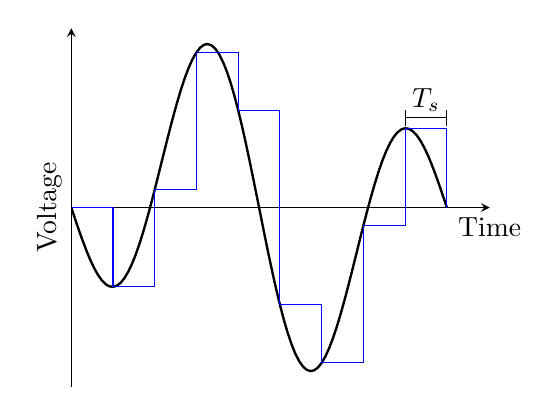
\begin{tikzpicture}
\begin{axis}[scale=0.8,
ticks=none,
%ymajorticks=false,
%xtick={3.1416,6.2832},
%xticklabels={$\pi$,$2\pi$},
unit vector ratio*=1 1 1,
xmin=0,
ymin=-3,
xmax=7,
ymax=3,
axis lines=middle,
x label style={at={(axis cs:7,0)},anchor=north},
y label style={at={(axis cs:0,0)},anchor=south,rotate=90},
xlabel=Time,
ylabel=Voltage]
\addplot[black,mark=none,samples=100,domain=0:6.2832,line width=0.3mm]{sin(deg(x))-2*sin(deg(2*x))};
\addplot[const plot,blue,mark=non]coordinates{(0,0)(0.6981,-1.3268)(1.3963,0.3008)(2.0944,2.5981)(2.7925,1.6276)(3.4907,-1.6276)(4.1888,-2.5981)(4.8869,-0.3008)(5.5851,1.3268)(6.2832,0)};
\draw[|-|](axis cs:5.5851,1.5)--(axis cs:6.2832,1.5);
\node at(axis cs:5.9342,1.8){$T_s$};
\end{axis}
\end{tikzpicture}
\caption{Voltage of input analogue signal (black) and of output analogue signal (blue). The input signal is held by a S\&H circuit for $T_s$.}
\label{fig:S/H}
\end{figure}
The S\&H circuit must sample at a sufficiently high frequency as specified by theorem \ref{sampling_theorem}.

\subsubsection{Quatization}
Quantization is the process of discretizing analogue signal values to discrete values and is done with an analogue-to-digital converter. Digital processors are incapable of dividing an interval into infinitely many subintervals (points), which means that a finite number of intervals has to be used. When an analogue signal is quantized its value is compared to a finite number of analogue values, rounded to the nearest value and expressed in digital numbering (binary). The number of digital values therefore depends on the number of bits dedicated to representing a given analogue value as a digital number. When rounding the analogue value to a digital value a round off error is produced, which can be decreased by increasing the number of possible digital values in the interval \cite{pelgrom}. Figure \ref{fig:quant} shows the graph of an analogue signal alongside the quantization levels.
\begin{figure}[H]
\centering
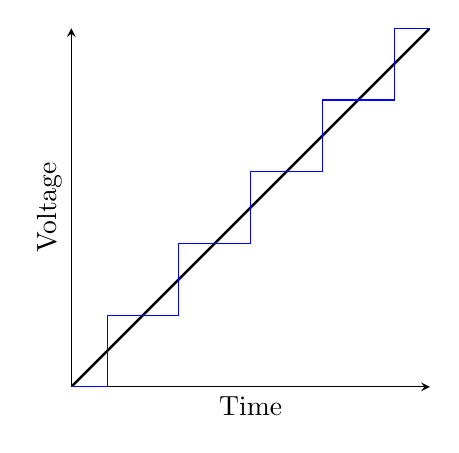
\begin{tikzpicture}
\begin{axis}[scale=0.8,
unit vector ratio*=1 1 1;
clip=false,
ticks=none,
axis lines=middle,
xmin=0,
ymin=0,
ymax=1,
xmax=1,
x label style={at={(axis cs:0.5,0)},anchor=north},
y label style={at={(axis cs:0,0.5)},rotate=90,anchor=south},
xlabel=Time,
ylabel=Voltage]
\draw[line width=0.3mm,black](axis cs:0,0)--(axis cs:1,1);
\addplot[const plot,no marks,blue]coordinates{(0,0)(0.1,0.2)(0.3,0.4)(0.5,0.6)(0.7,0.8)(0.9,1)(1,1)};
\end{axis}
\end{tikzpicture}
\caption{Plot of continuous levels of voltage (V) versus time (black) and the quantized voltage levels (blue) expressed in least significant bit (LSB) multiplied by sensitivity (V/LSB).}
\label{fig:quant}
\end{figure}

There exist different ADCs \cite{pelgrom} all with the purpose of expressing a continuous analogue signal as a discrete and quantized digital signal. These different approaches will  not be described as the above description will make do for now. The process of sampling described in section \ref{sec:sampling} will be done with an ADC in the experiments later in the project.

\clearpage
\section{Signals and noise}
This project has the purpose of measuring sound signals and process it in an advantageous way so as to be able to produce a spectrogram of said signal. It is therefore necessary to clarify what is meant by a signal and which kinds of signals are likely to be encountered.

\subsection{Signals}
A signal is ``[\dots]\textit{a means of conveying information}[\dots]'' \cite{signal_noise} and is in this project a sound signal consisting of sound waves from a musical instrument propagating in a medium (air) and measured by a membrane in a microphone and thereafter converted to an analogue voltage. As sound waves from musical instruments are no different than any other kind of sound waves they will all be measured by the microphone. These other sound waves will be referred to as \textit{noise}.

\subsection{Noise}
This section is mainly inspired by chapter 2 in \cite{signal_noise}. \\ \\
Noise is any measured interference of a signal conveying information and is merely another signal measured alongside the wanted signal, where the noise carries information about the source of the noise.  Noise is generally thought of as unwanted as it can be hard to distinguish the signal from it and therefore extract the wanted information. Noise is present in almost all measurements of any signal, and any measurement of a signal must therefore take this into consideration as noise limits the usability of measurements by
\begin{itemize}
\item reducing the accuracy of signal processing systems.
\item reducing the accuracy of decision making by pattern recognition.
\end{itemize}
The ability to counter noise depends on knowledge of the specific noise so as to be able to use the characteristics of the noise to distinguish it and the wanted signal from each other.
\\ \\
In this project the noise is characterized as being \textit{acoustic noise}. There are two such kinds:
\begin{enumerate}
\item \textit{Additive acoustic noise} \\
Noise from moving or colliding objects. This is generally any disturbing signal stemming form outside of the system to be measured.
\item \textit{Acoustic feedback noise} \\
Noise due to echo or feedback. This includes reflections of sound waves on objects and feedback by coupling of microphones and speakers.
\end{enumerate}

In addition to this noise is categorized by the characteristic of the spectrum of the noise:
\begin{itemize}
\item \textit{White noise}\\
Purely random noise with a constant power spectrum; all frequencies occur equally.
\item \textit{Bandlimited (white) noise}\\
Bandlimited noise. White noise bandlimited in a spectrum that covers the spectrum of the interferred signal acts as true white noise with respect to the signal.
\item \textit{Coloured noise}\\
Any non-white noise; noise which does not have a constant power spectrum.
\end{itemize}

As noise reduction is generally wanted, this project will also seek to eliminate it by recording music in an anechoic rum. Playing a pitch alone in an anechoic room is a way of minimizing noise factors. There are many different noise sources from e.g. the surrounding environment, electrical equipment, other people and even the instrument playing itself since it is difficult to make a pure tone by an acoustic sound source such as a guitar. A pure tone is a sinusoidal waveform consisting of a single frequency and may therefore be difficult to play on an instrument \cite{AcousticNoise}. Usually, sound is reflected off the walls in a room which is also a source of noise. This is a form of convolution and is minimized in the anechoic room because sound is absorbed by the walls. Moreover, due to the construction of the anechoic room, noise from e.g. bypassing cars is also minimized, and the sound may be recorded with a minimum of hardware, which otherwise may also produce noise.
\\ \\
The music used in this project will therefore be recorded in an anechoic room because the noise is minimized. 
It is not expected that musicians using the system in the future have access to an anechoic room as well but if the system doesn't work with sounds recorded in the anechoic room then it with most certainty doesn't work at other places neither. \chr{Hvad skal der stå her (utydelig)} However, in order to reproduce the conditions of a typical musician working around other people, background noise can also be made in the anechoic room but should of course not drown the music. This form of noise is additive whereas e.g. noise reflected off walls as mentioned above is a convolution of the noise and the original signal. In general, convolution noise depends on the state of the system whereas additive noise does not.
\frede{Tilføj matematisk beskrivelse af støj.}

\subsection{SNR}
Signal-to-noise ratio is a measure of the amount of noise in a signal.
\begin{definition}
The signal-to-noise ratio (SNR) of a signal and noise is defined as
\begin{equation}\label{def:SNR}
	SNR=10\log_{10}\left(\frac{\sigma_{signal}^2}{\sigma_{noise}^2}\right)
\end{equation}
where $\sigma_{signal}^2$ is the variance of the signal and $\sigma_{noise}^2$ is the variance of the noise [\textbf{page 229}\cite{DTSP}].
\end{definition}
To calculated the variances of the signal and noise the standard deviation $\sigma$ can be calculated and if the input signal has mean = 0 the standard deviation of the signal can be calculated by the root mean square (RMS) of the signal [\textbf{page 228}\cite{DTSP}] which is defined as
\begin{align}\label{eq:RMS}
	x_{rms} 
	&=\sqrt{\frac{1}{n} \sum_{i=1}^n x_i^2}\\
	&= \sqrt{\frac{x_1^2 + x_2^2 + \dots + x_n^2}{n}}.
\end{align}





